
\documentclass[submit]{harvardml}

% Put in your full name and email address.
\name{Luke Mueller}
\email{lam908@mail.harvard.edu}

% List any people you worked with.
\collaborators{%
  John Doe,
  Fred Doe
}

% You don't need to change these.
\course{CS181-S16}
\assignment{Assignment \#4}
\duedate{5:00pm Feb 1, 2016}

\usepackage[OT1]{fontenc}
\usepackage[colorlinks,citecolor=blue,urlcolor=blue]{hyperref}
\usepackage[pdftex]{graphicx}
\usepackage{subfig}
\usepackage{fullpage}
\usepackage{palatino}
\usepackage{mathpazo}
\usepackage{amsmath}
\usepackage{amssymb}
\usepackage{color}
\usepackage{todonotes}
\usepackage{listings}
\usepackage{common}
\usepackage{bm}
\usepackage[normalem]{ulem}
\useunder{\uline}{\ul}{}

\usepackage[mmddyyyy,hhmmss]{datetime}

\definecolor{verbgray}{gray}{0.9}

\lstnewenvironment{csv}{%
  \lstset{backgroundcolor=\color{verbgray},
  frame=single,
  framerule=0pt,
  basicstyle=\ttfamily,
  columns=fullflexible}}{}

\begin{document}
\begin{center}
{\Large Homework 4: Clustering}\\
\end{center}

There is a mathematical component and a programming component to this homework.
Please submit ONLY your PDF to Canvas, and push all of your work to your Github
repository. If a question requires you to make any plots, please
include those in the writeup.


%%%%%%%%%%%%%%%%%%%%%%%%%%%%%%%%%%%%%%%%%%%%%
% Problem 1
%%%%%%%%%%%%%%%%%%%%%%%%%%%%%%%%%%%%%%%%%%%%%
\begin{problem}[The Curse of Dimensionality, 4pts]
In~$d$ dimensions, consider a hypersphere of unit radius, centered at zero,
which is inscribed in a hypercube, also centered at zero, with edges of length
two.  What fraction of the hypercube's volume is contained within the
hypersphere?  Write this as a function of~$d$.  What happens when~$d$ becomes
large?
\end{problem}
\subsection*{Solution}

Volume of the hypercube with dimensions $d$ and edge length $2x$: $V_c = (2x)^d$ \\
Volume of the hypersphere with dimensions $d$ and radius $x$: $V_s = \frac{S_d}{d} * x^d$ where $S_d = \frac{2\pi^{d/2}}{\Gamma(d/2)}$ \\ 

\noindent
We are interested in the fraction $V_s / V_c$, which expanded by the terms above is:

\[
\frac{V_s}{V_c} = \frac{2\pi^{d/2}}{\Gamma(d/2)} * \frac{x^d}{d} * \frac{1}{(2x)^d} = \frac{2\pi^{d/2}}{\Gamma(d/2)} * \frac{1}{2^dd}
\]

\noindent
Then we manipulate the solution using Stirling's formula for the Gamma function, $\Gamma \left({x + 1}\right) = \sqrt {2 \pi x} \, x^x \exp^{-x}$ \\

In particular: $\Gamma(d/2) = \Gamma(d/2-1+1) = 2\pi^{1/2}\exp^{-d/2+1}(d/2-1)^{d/2-1/2}$ \\

\noindent
Thus we have:

\begin{align*}
\frac{\pi^{d/2}}{2^{d-1}\times d(2\pi)^{1/2} \times \exp^{-d/2+1} \times \frac{d-2}{2}^{(d-1)/2}} & =
\frac{\pi^\frac{d-1}{2} \times \pi^\frac{1}{2}}{\pi^{1/2} \times 2^{d-1+1/2} \times d \times \exp^{-(d-1)/2} \times \exp^{1/2} \times \frac{d-2}{2}^{(d-1)/2}} \\
& = \frac{1}{\big(\frac{d-2}{2\pi\exp}\big)^\frac{d-1}{2} \times 2^{(d-1/2)} \times d \times \exp^{1/2}}
\end{align*}

\noindent
Then taking the limit as $d \rightarrow \infty$ the fraction $\frac{V_s}{V_c} = 0$. Thus, at high dimensions the volume of the hypersphere $V_s$ becomes negligible in comparison to the volume of the hypercube, $V_c$. This further implies that most of the volume held by the hypercube $V_c$ is contained in its corners rather than its center.

\newpage
\begin{problem}[Norms, Distances, and Hierarchical Clustering, 5 pts]

  Consider the following four data points, belonging to three clusters: the
  black cluster $((x_1, y_1) = (0.1, 0.5) $ and $(x_2, y_2) = (0.35, 0.75))$,
  the red cluster $(x_3, y_3) = (0.28, 1.35)$ cluster, and the blue cluster
  $(x_4, y_4) = (0, 1.01)$.

  \begin{center} 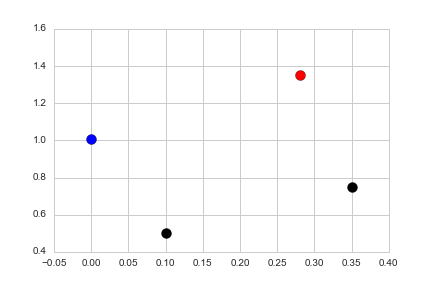
\includegraphics[scale=.4]{scatterplot.png} \end{center}
  At each step of hierarchical clustering, the two most similar (or least
  dissimilar) clusters are merged together. This step is repeated until there is
  one single group. Different distances can be used to measure group
  dissimilarity. Recall the definition of the $l_1$, $l_2$, and $l_{\infty}$
  norm:
  \begin{itemize}
    \item For $\mathbf{x} \in \mathbb{R}^n, \| \mathbf{x} \|_1 = \sum_{i = 1}^n
      |x_i|$
    \item For $\mathbf{x} \in \mathbb{R}^n, \| \mathbf{x} \|_2 = \sqrt{\sum_{i =
      1}^n x_i^2 }$
    \item For $\mathbf{x} \in \mathbb{R}^n, \| \mathbf{x} \|_{\infty} = \max_{i
      = 1}^n |x_i|$
  \end{itemize}
  Also recall the definition of single-link distance, complete-link distance,
  and average-link distance between two clusters:
  \begin{itemize}
    \item Single-link clustering: for clusters $G$ and $H$, $d_{S}(G, H) =
    \min_{i \in G, j\in H} d(i, j)$
    \item Complete-link clustering: for clusters $G$ and $H$, $d_{C}(G, H) =
    \max_{i \in G, j\in H} d(i, j)$
    \item Average-link clustering: for clusters $G$ and $H$, $d_{A}(G, H) =
      \frac{1}{|G| |H|} \sum_{i\in G}\sum_{j \in H} d(i, j)$
  \end{itemize}
  \paragraph{Warm up question.} \noindent Draw the 2D unit sphere for each norm,
  defined as $\mathcal{S} = \{x \in \mathbb{R}^2: \|x\| = 1 \}$. Feel free to do
  it by hand, take a picture and include it in your pdf.

  \paragraph{Main question.}
  \noindent For each norm ($l_1, l_2, l_\infty$) and each clustering method
  (single, complete, or average link clustering), specify which 2 clusters would
  be the first to merge.
\end{problem}

\subsection*{Solution}

\begin{center} 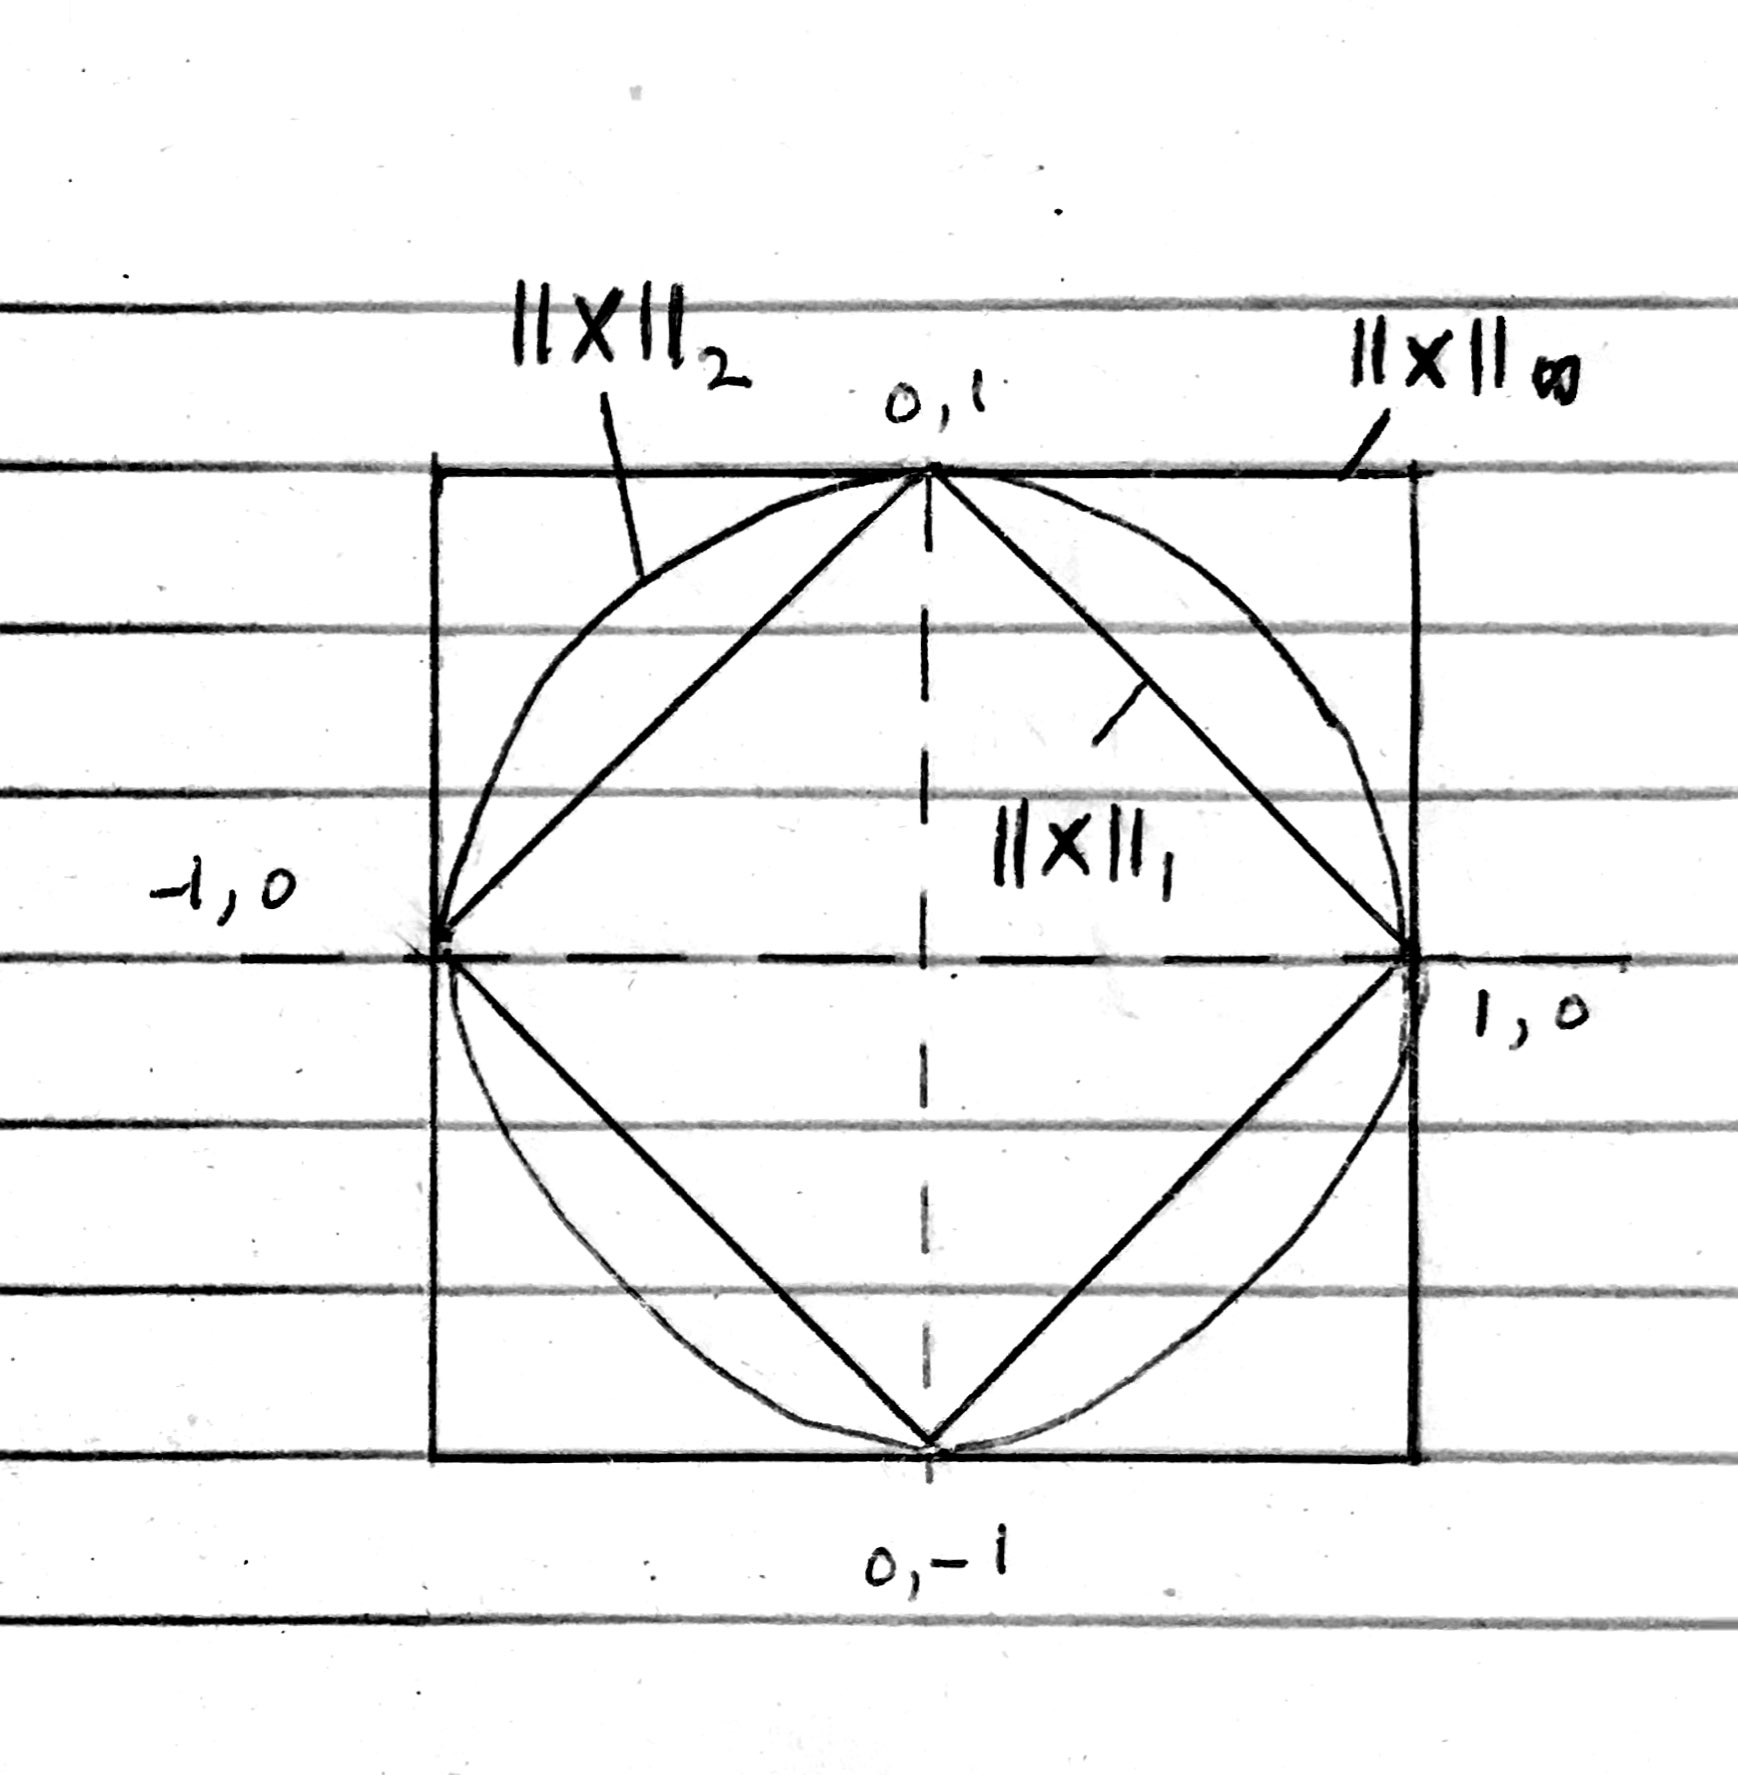
\includegraphics[scale=.15]{norms.jpg} \end{center}

\begin{table}[htb]
	\centering
	\caption{Main Question Results}
	\label{my-label}
	\begin{tabular}{lccc}
		\multicolumn{1}{c}{{\ul }} & {\ul $L_1$}             & {\ul $L_2$}             & {\ul $L_\infty$}         \\
		\textbf{Comparison}        & \multicolumn{1}{l}{} & \multicolumn{1}{l}{} & \multicolumn{1}{l}{} \\
		\textit{1 vs. 3}           & 1.03                 & 0.869                & 0.85                 \\
		\textit{2 vs. 3}           & 0.67                 & 0.604                & 0.60                  \\
		\textit{1 vs. 4}           & 0.61                 & 0.520                & 0.51                 \\
		\textit{2 vs. 4}           & 0.61                 & 0.436                & 0.35                 \\
		\textit{3 vs. 4}           & 0.62                 & 0.440                & 0.34                 \\
		& \multicolumn{1}{l}{} & \multicolumn{1}{l}{} & \multicolumn{1}{l}{} \\
		\textbf{Averages}          & \multicolumn{1}{l}{} & \multicolumn{1}{l}{} & \multicolumn{1}{l}{} \\
		\textit{Black and Blue}    & 0.61                 & 0.48                 & 0.43                 \\
		\textit{Black and Red}     & 0.85                 & 0.74                 & 0.73                 \\
		&                      &                      &                      \\
		\textbf{Clustering algorithm results}        &                      &                      &                      \\
		\textit{Single}            & Black and Blue       & Black and Blue       & Blue and Red         \\
		\textit{Complete}          & Black and Blue       & Blue and Red        & Blue and Red         \\
		\textit{Average}           & Black and Blue       & Blue and Red        & Blue and Red        
	\end{tabular}
\end{table}

Table 1 shows the distances between points under the 3 specified norms, the $L_1$ norm, the $L_2$ norm, and the $L_\infty$ norm. Importantly, points 1 and 2 belong to the black cluster, point 3 belongs to the red cluster, and point 4 belongs to the blue cluster. The "Averages" heading gives the averaged euclidean distance between the black cluster, and either the blue or red cluster (both having only 1 point each) for use in the Average-link clustering calculation.

After the distances were calculated, the 2 clusters first to merge under the 3 clustering algorithms were determined as follows (and are summarized in the table above). The single link clustering algorithm preferred the minimum distance between any two points. Under the $L_1$ norm, both points in the black cluster were equidistant from the blue cluster ($d = 0.61$), thus the black and blue cluster merged first. Under the $L_2$ norm, the minimum distance was between points 2 and 4 ($d = 0.436$), thus the black and blue cluster again merged first. Under the $L_\infty$ norm, the minimum distance was between points 3 and 4 ($d = 0.34$), thus the blue and red cluster merged first. 

The complete-link clustering algorithm was similar to the single-link clustering algorithm, except for the black cluster, which took the maximum distance between points of other clusters first, before seeking the minimum distance. Under the $L_1$ norm, the result was the same as above, since the distance from the black cluster to the blue cluster was the same for points 1 and 2. Under the $L_2$ norm, the blue and red clusters merged first ($d=0.440$), since the maximum distance between the black and blue cluster was 0.520. Under the $L_\infty$ norm, the result was the same as above. 

The average-link clustering algorithm was similar to the above clustering algorithms, except for the black cluster, which averaged its distances with the other clusters. The values of these averages are given in the table above, as well as the results of the clustering algorithm. 

\newpage

\section*{K-Means [15 pts]}
Implement K-Means clustering from scratch.\footnote{That is, don't use a
third-party machine learning implementation like \texttt{scikit-learn};
\texttt{numpy} is fine.}. You have been provided with the MNIST dataset. You can
learn more about it at  \url{http://yann.lecun.com/exdb/mnist/}. The MNIST task
is widely used in supervised learning, and modern algorithms with neural
networks do very well on this task. We can also use MNIST for interesting
unsupervised tasks. You are given representations of 6000 MNIST images, each of
which are $28\times28$  handwritten digits. In this problem, you will implement
K-means clustering on MNIST, to show how this relatively simple algorithm can
cluster similar-looking images together quite well.

\begin{problem}[K-means, 15pts]
The given code loads the images into your environment as a 6000x28x28 array.
Implement K-means clustering on it for a few different values of $K$, and show
results from the fit. Show the mean images for each class, and by selecting a
few representative images for each class. You should explain how you selected
these representative images. To render an image, use the numpy imshow function,
which the distribution code gives an example of. Use squared norm as your
distance metric. You should feel free to explore other metrics along with
squared norm if you are interested in seeing the effects of using those. Also,
your code should use the entire provided 6000-image dataset (which, by the way,
is only 10\% of the full MNIST set).

Are the results wildly different for different restarts and/or different $K$?
Plot the K-means objective function as a function of iteration and verify that
it never increases.

Finally, implement K-means++ and see if gives you more satisfying
initializations (and final results) for K-means. Explain your findings.

As in past problem sets, please include your plots in this document. There may
be tons of plots for this problem, so feel free to take up multiple pages, as
long as it is organized.
\end{problem}

\subsection*{Solution}

The following pages show results from the K means algorithm under different hyperparameter settings. In particular, the function allows different inputs for $K$: the number of clusters, $D$: the number of representative images selected for each cluster, and K-means ++: specification of the cluster initialization process. The mean images figures are the $K$ centroids, and the representative images figures are the $D$ closest inputs to each $K$ centroid, where "closeness" is measured by the minimum squared norm. 

Setting $K$ to different values had significant results on the algorithm output, irrespective of cluster initialization or $D$. Under smaller numbers of clusters, the algorithm had greater difficulty differentiating images. For example, under $K=2$ (see figures 4-6, 10-12), the mean clusters vaguely represented numbers $8$ and $9$, since 8 was similar to 0s and 5s, and 9 was similar to 1s and 4s. Numbers like 2 or 6 were not predicted at all since their figures are more unique in the sample. Increasing $K$ to 10 captured all types of numbers in the sample, though there were errors in the representative images for numbers with similar figures (i.e., 4, 7, and 9). Increasing $K$ to 20 (figure 14) attenuated some of these errors, but there were still misclassified images for numbers with similar figures.

Specifying different processes for initializing the clusters did not have substantial effects on the output (mean or representative images), though the K-Means ++ initialization drastically reduced the required iterations for convergence. For example, under $K=2$ and a naive initialization scheme (picking 10 images from the sample at random), the algorithm required 84 iterations and had an initial objective function value of $1.7\times 10^{10}$. By contrast, under $K=2$ and the K-Means ++ initialization scheme (choosing 10 images based on inverse probability sampling as a function of distance), the algorithm required 30 iterations and had an initial objective function value of $1.98\times 10^{10}$. Similar results were found under different values of $K$ and $D$. 

Finally, $\textbf{all}$ objective function plots show that the objective function value decreases with subsequent iterations, thus by minimizing the loss the algorithm approaches convergence. 

\newpage

\begin{figure}
	\centering
	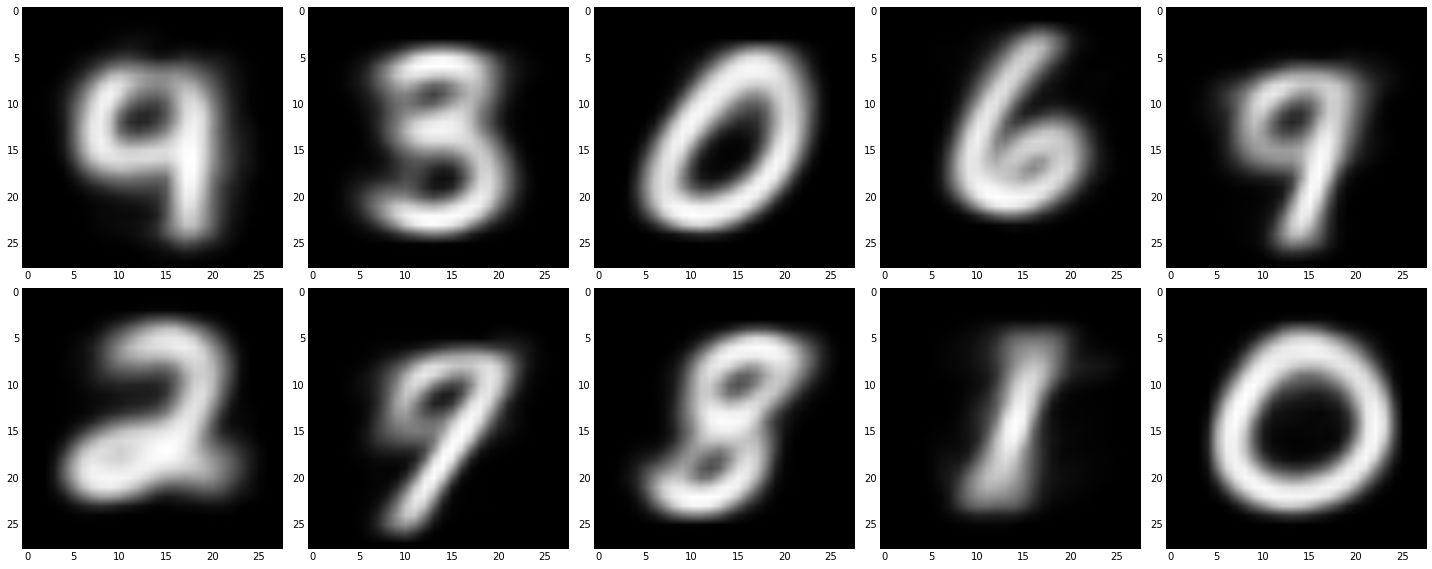
\includegraphics[width=0.6\textwidth]{output_11_0.png}
	\caption{Mean images for each class: $K = 10$, naive cluster initialization }
\end{figure}

\begin{figure}
	\centering
	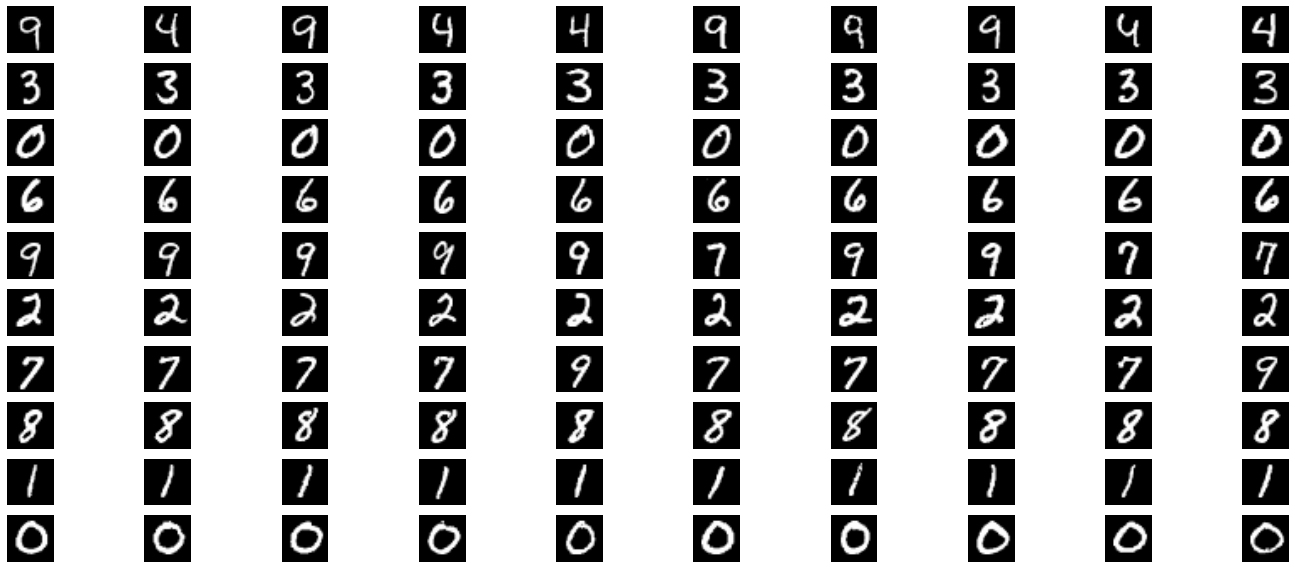
\includegraphics[width=1.0\textwidth]{output_11_1.png}
	\caption{Representative images for each class: $K = 10$, $D = 10$, naive cluster initialization }
\end{figure}

\begin{figure}
	\centering
	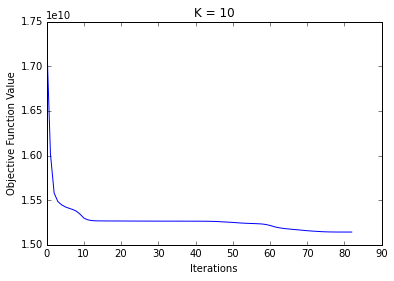
\includegraphics[width=0.6\textwidth]{output_12_0.png}
	\caption{Objective function minimization: $K = 10$, naive cluster initialization }
\end{figure}

%

\begin{figure}
	\centering
	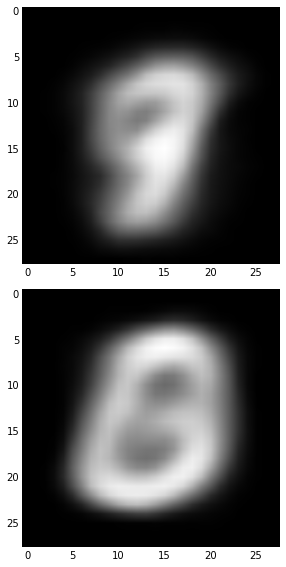
\includegraphics[height=0.4\textwidth]{output_14_0.png}
	\caption{Mean images for each class: $K = 2$, naive cluster initialization }
\end{figure}

\begin{figure}
	\centering
	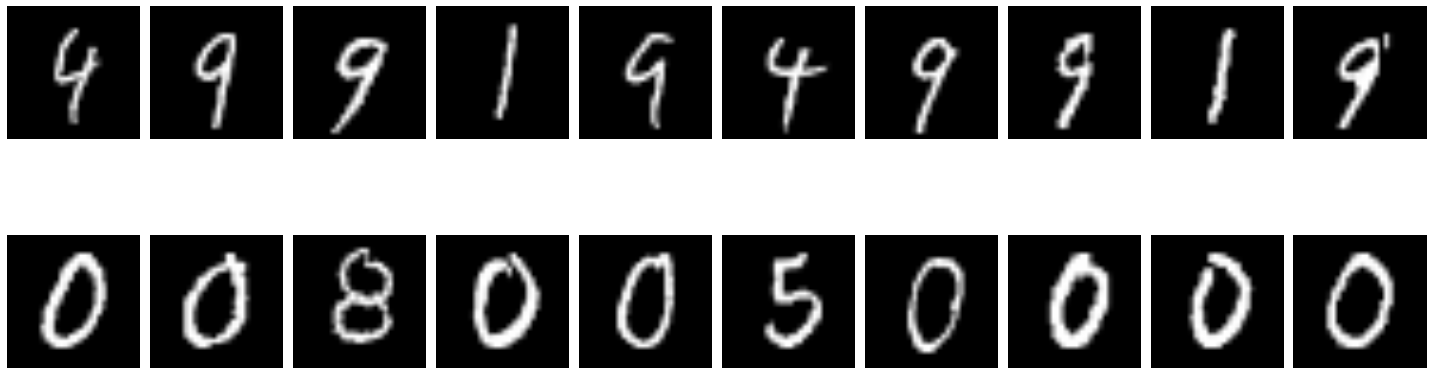
\includegraphics[width=1.0\textwidth]{output_14_1.png}
	\caption{Representative images for each class: $K = 2$, $D = 10$, naive cluster initialization }
\end{figure}

\begin{figure}
	\centering
	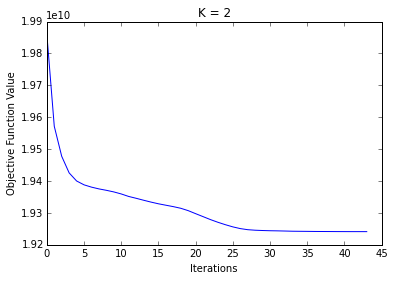
\includegraphics[width=0.6\textwidth]{output_15_0.png}
	\caption{Objective function minimization: $K = 2$, naive cluster initialization }
\end{figure}

% K means ++ diagrams

\begin{figure}
	\centering
	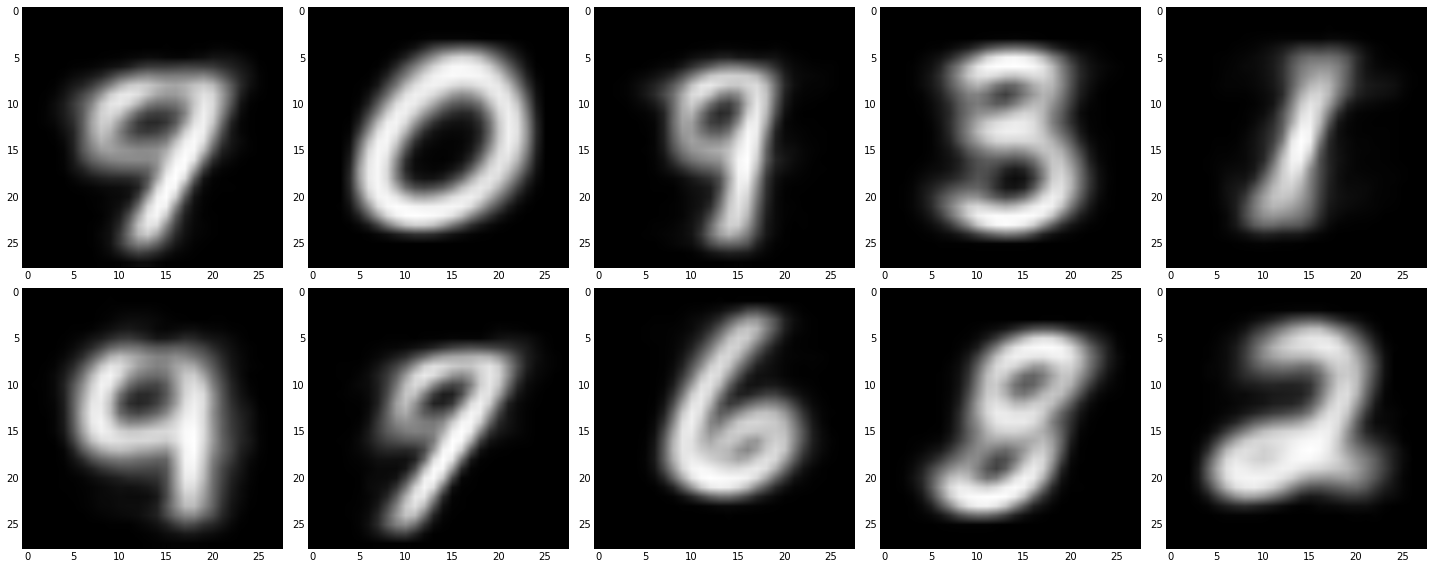
\includegraphics[width=0.6\textwidth]{output_2_0.png}
	\caption{Mean images for each class: $K = 10$, K-means ++ cluster initialization }
\end{figure}

\begin{figure}
	\centering
	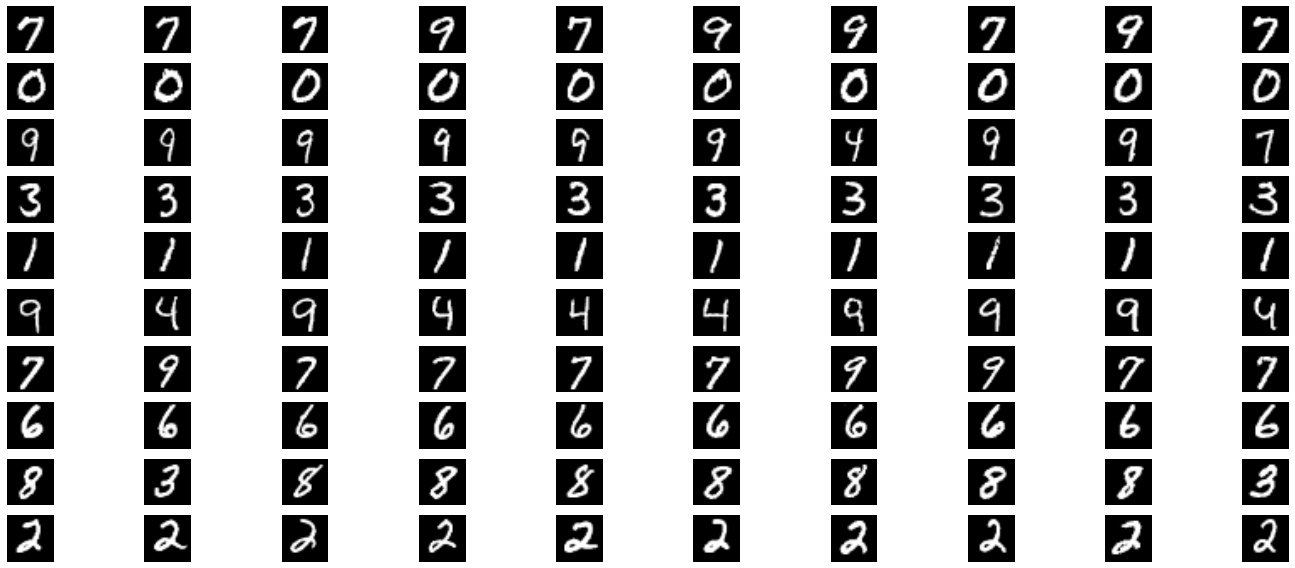
\includegraphics[width=1.0\textwidth]{output_2_1.png}
	\caption{Representative images for each class: $K = 10$, $D = 10$, K-means ++ cluster initialization }
\end{figure}

\begin{figure}
	\centering
	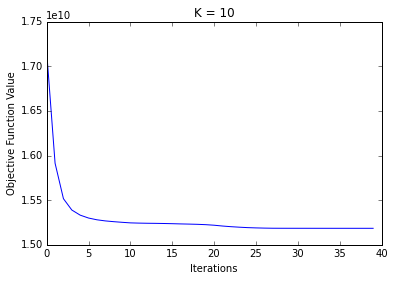
\includegraphics[width=0.6\textwidth]{output_3_0.png}
	\caption{Objective function minimization: $K = 10$, K-means ++ cluster initialization }
\end{figure}

%

\begin{figure}
	\centering
	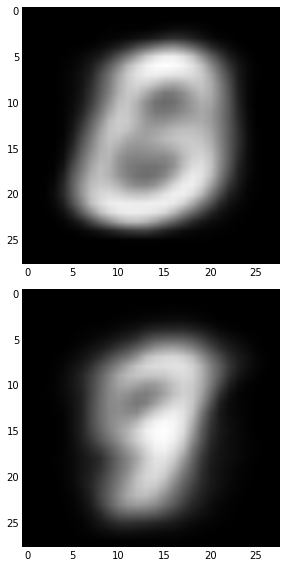
\includegraphics[height=0.4\textwidth]{output_5_0.png}
	\caption{Mean images for each class: $K = 2$, K-means ++ cluster initialization }
\end{figure}

\begin{figure}
	\centering
	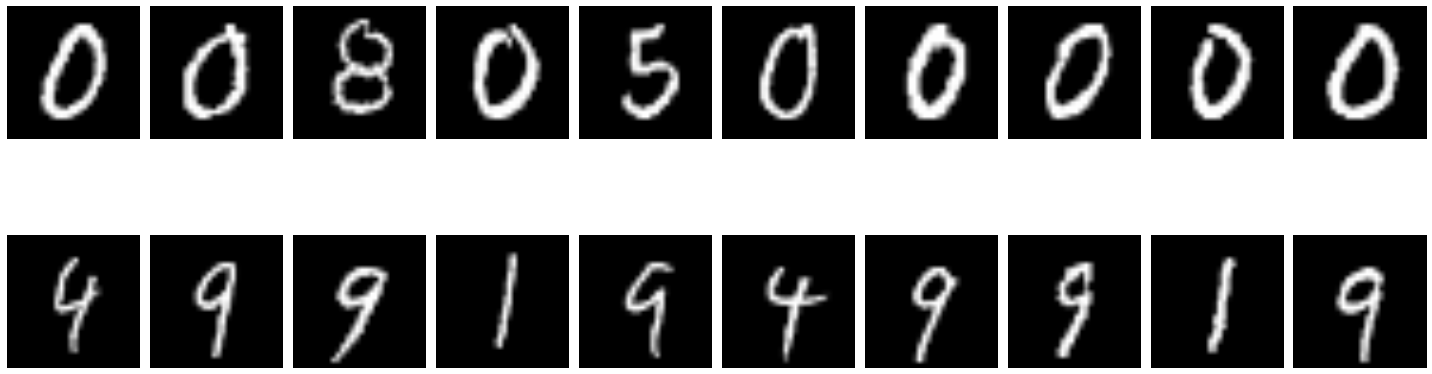
\includegraphics[width=1.0\textwidth]{output_5_1.png}
	\caption{Representative images for each class: $K = 2$, $D = 10$, K-means ++ cluster initialization }
\end{figure}

\begin{figure}
	\centering
	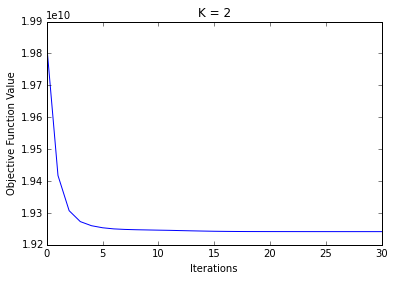
\includegraphics[width=0.6\textwidth]{output_6_0.png}
	\caption{Objective function minimization: $K = 2$, K-means ++ cluster initialization }
\end{figure}

%

\begin{figure}
	\centering
	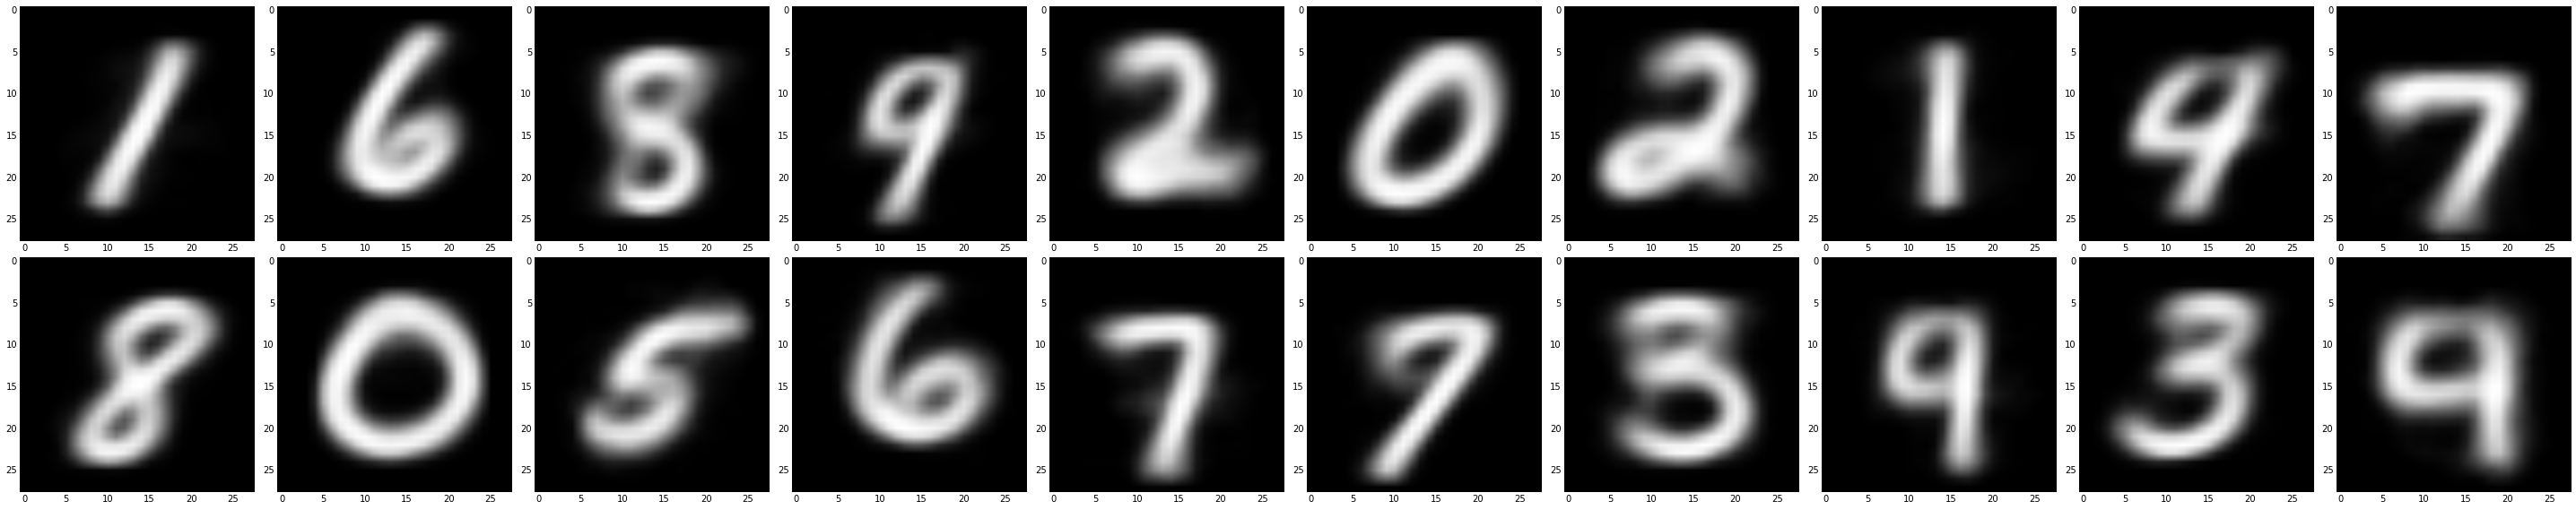
\includegraphics[width=0.6\textwidth]{output_8_0.png}
	\caption{Mean images for each class: $K = 20$, K-means ++ cluster initialization }
\end{figure}

\begin{figure}
	\centering
	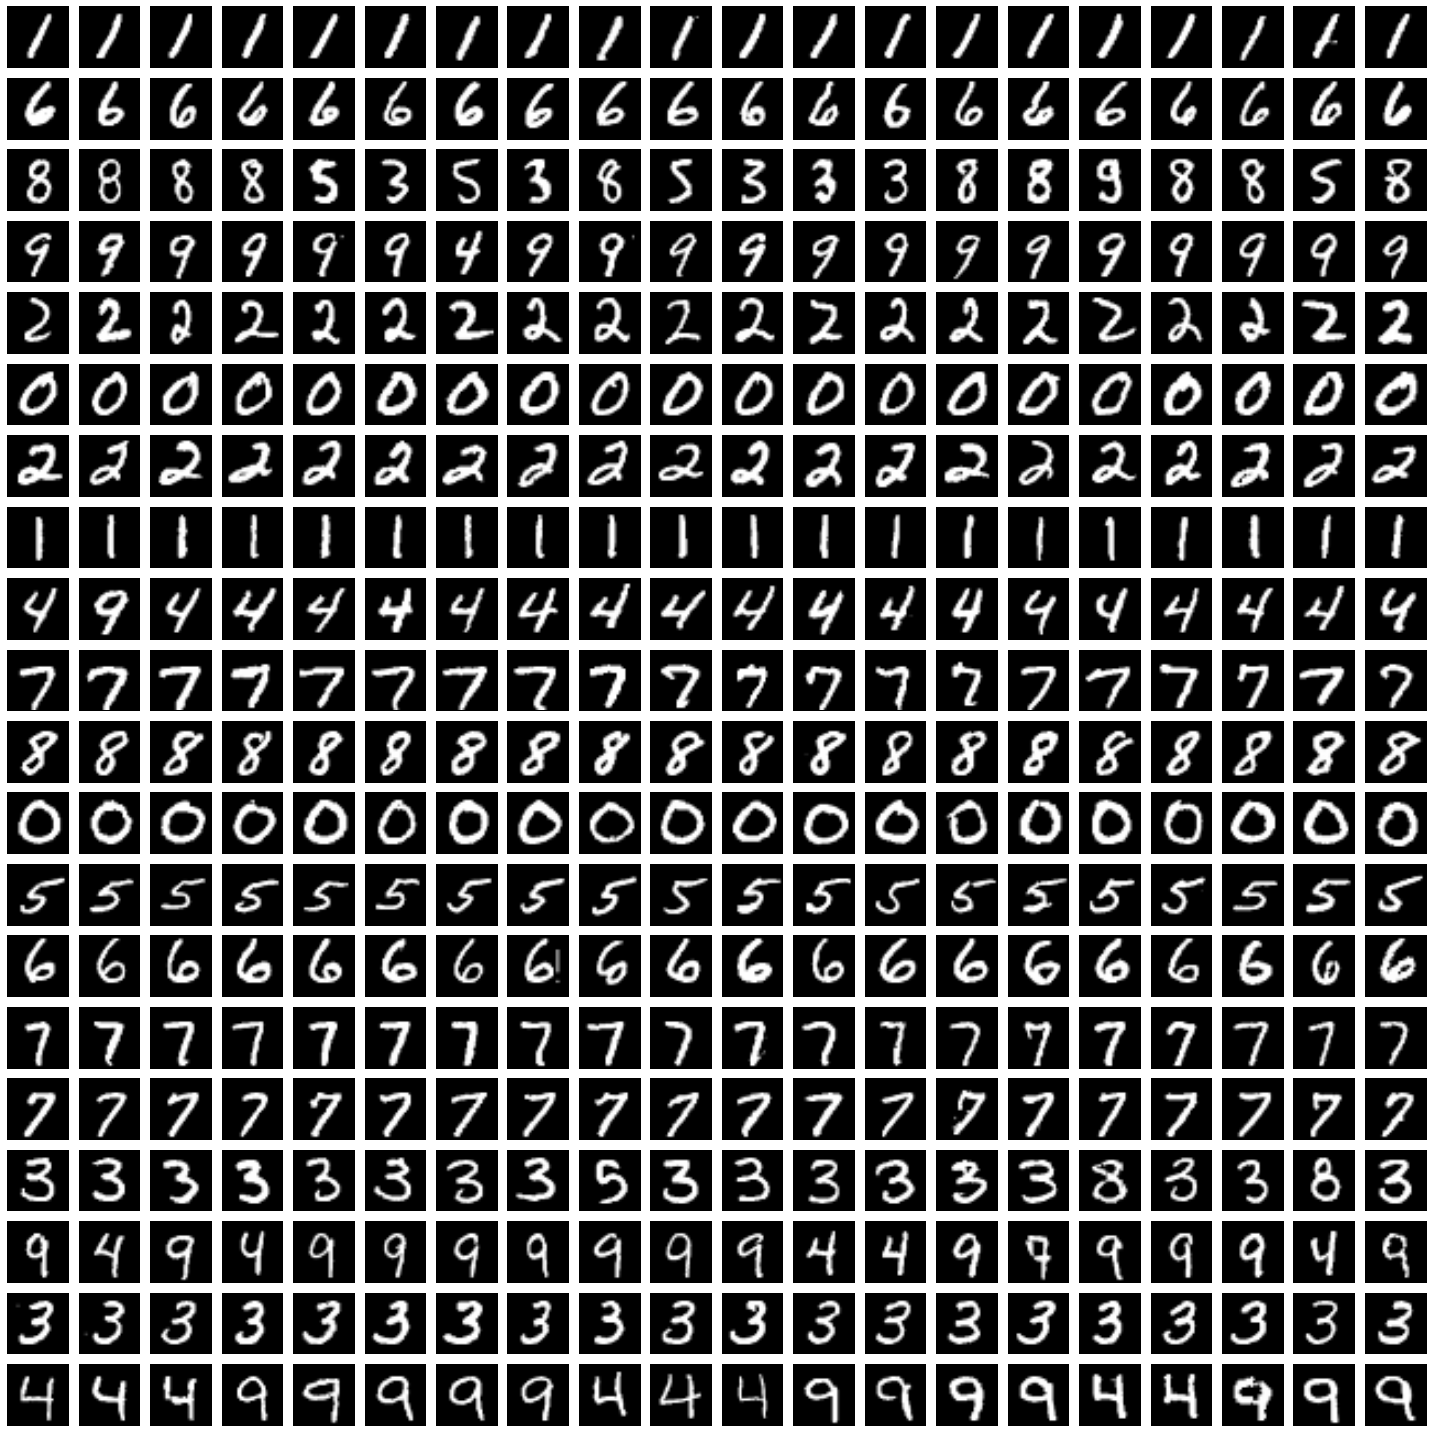
\includegraphics[width=1.0\textwidth]{output_8_1.png}
	\caption{Representative images for each class: $K = 20$, $D = 20$, K-means ++ cluster initialization }
\end{figure}

\begin{figure}
	\centering
	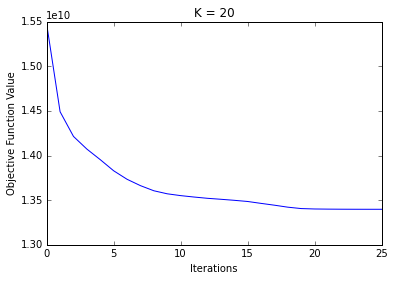
\includegraphics[width=0.6\textwidth]{output_9_0.png}
	\caption{Objective function minimization: $K = 20$, K-means ++ cluster initialization }
\end{figure}

%Figure out how to load it into your environment and turn it into a set of
%vectors.  Run K-Means on it for a few different~$K$ and show some results from
%the fit.  What do the mean images look like?  What are some representative
%images from each of the clusters?  Are the results wildly different for
%different restarts and/or different~$K$?  Plot the K-Means objective function
%(distortion measure) as a function of iteration and verify that it never
%increases.

%\subsection*{4. Implement K-Means++ [4 pts]} mplement K-Means++ and see if it
%gives you more satisfying initializations for K-Means.  Explain your findings.

\clearpage
\begin{problem}[Calibration, 1pt]
Approximately how long did this homework take you to complete?
\end{problem}

10 hours.

\end{document}
